\documentclass[a4paper,11pt]{article}
\usepackage[utf8]{inputenc}
\usepackage[T2A]{fontenc}
\usepackage[russian]{babel}
\usepackage{hyperref}
\usepackage{booktabs}
\usepackage{geometry}
\usepackage{makecell}
\usepackage{graphicx}
\usepackage{amsmath}
\geometry{left=2cm,right=2cm,top=2cm,bottom=2cm}

\title{%
  LLM‑compressor. Отчёт\\[0.5ex]
  {\large\itshape Итоговый проект курса Deep Learning School}%
}
\author{%
  Студент: Матюнина Юлия Алексеевна\\
  Руководитель: Алексей Дмитриевич Рухович%
}
\date{}

\begin{document}
\maketitle

\section*{Введение}

Данная работа сделана к качестве итогового проекта курса от Deep Learning School.

Необходимо было на базе LLM с помощью алгоритма арифметической компрессии реализовать архиватор текста. Сжать Википедию и посчитать её объём. Улучшить коэффициент компрессии с помощью prefix tuning или steering. Обучить модель генерировать распределение для steering-вектора, чтобы ещё сильнее улучшить компрессию.

Основная часть работы находится в ноутбуках \texttt{Compression with different models.ipynb}, \texttt{Compression with steering vector.ipynb} и \texttt{Steering vector with hyper prior.ipynb}.

В ходе нашего исследования было провидено сравнение качества и скорости арифметического кодирования и декодирования с использованием различных небольших LLM. Были проведены эксперименты с использованием steering vector - фиксированного и обучаемого.
Также сам steering vector кодировался с помощзью различных видов hyper-prior.

\section*{Подготовка}

При подготовке работы были изучены научные статьи
\begin{itemize}
  \item \href{https://arxiv.org/pdf/2309.10668}{Language Modeling is Compression},
  \item \href{https://arxiv.org/pdf/1802.01436}{Variational image compression with a scale hyperprior}.
\end{itemize}
Для сжатия используется датасет Wikipedia
\href{https://www.kaggle.com/datasets/nightfury1103/enwik8}{Enwik8}.

Запуск моделей производился на Colab с использованием графического процессора T4.

\section{Арифметическое кодирование с LLM}

\textbf{Арифметическое кодирование} — метод энтропийного сжатия, в котором вся последовательность токенов кодируется как одно число в интервале \([0,1)\). Границы интервала постепенно сужаются в соответствии с предсказанным LLM распределением.

\subsection*{Алгоритм}

\begin{enumerate}
  \item \textbf{Инициализация.} Устанавливаем
  \[
    \texttt{low} = 0,\qquad
    \texttt{high} = 2^{\text{precision}} - 1.
  \]

  \item \textbf{Основной цикл} (для каждого токена \(t_i\)):
  \begin{enumerate}
    \item \emph{Предсказание.} По префиксу \((t_0,\dots,t_{i-1})\) LLM выдаёт
    \[
      \text{probs}=[p_0, p_1, \dots, p_{V-1}],\quad \sum_{k=0}^{V-1}p_k=1.
    \]

    \item \emph{Кумулятивная функция.}
    \[
      \text{CDF}[k] = \sum_{j<k} p_j,\quad \text{CDF}[V]=1.
    \]

    \item \emph{Сужение интервала.} Обозначим \(R = \texttt{high}-\texttt{low}\). Тогда
    \[
      \texttt{low}  \leftarrow \texttt{low}
        + \left\lfloor R \times \text{CDF}[t_i]\right\rfloor,
    \]
    \[
      \texttt{high} \leftarrow \texttt{low}
        + \left\lfloor R \times \text{CDF}[t_i+1]\right\rfloor.
    \]

    \item \emph{Нормализация.} При попадании границ в «экстремальные» биты (E1/E2/E3) выполняем битовый сдвиг для сохранения точности.
  \end{enumerate}

  \item \textbf{Завершение.} После кодирования всех токенов выбираем любое число внутри финального интервала \([\texttt{low},\texttt{high})\) и выводим его битовый префикс длины \(\text{precision}\).

  \item \textbf{Декодирование.}
  \begin{enumerate}
    \item Читаем первые \(\text{precision}\) бит как целое \(\texttt{value}\), инициализируем
    \(\texttt{low}=0,\ \texttt{high}=2^{\text{precision}}-1\).
    \item Для каждого токена \(t_i\):
    \begin{itemize}
      \item Находим такое \(t_i\), что
      \[
        \text{CDF}[t_i] \;\le\;\frac{\texttt{value}-\texttt{low}}{\texttt{high}-\texttt{low}}
        < \text{CDF}[t_i+1].
      \]
      \item Сужаем \(\texttt{low}\), \(\texttt{high}\) теми же формулами, что и в энкодере, и нормализуем.
    \end{itemize}
  \end{enumerate}
\end{enumerate}


\section*{Без чанков или с чанками}

В начале обоснуем необходимость разбиения на чанки при экспериментах. В этом разделе использовалась модель \texttt{EleutherAI/pythia-70m}. Но результаты будут схожими и для других моделей.

Всего сжималось 400\,000 бит информации (50\,кБ). Весь объём разбивался на части по 16\,000 бит (2\,кБ). Получается 25 чанков.
Ниже приведена сравнительная таблица результатов сжатия без использования чанков и с разбиением на чанки:

\begin{table}[ht]
\centering
\resizebox{\textwidth}{!}{%
  \begin{tabular}{lrrrr}
    \toprule
    Метод        & Время кодирования, с & Время декодирования, с & Размер после сжатия, бит & Коэффициент сжатия \\
    \midrule
    Без чанков   & 733.66               & 731.65                 & 60\,471                   & 0.1512             \\
    С чанками    & 138.17               & 152.33                 & 66\,303                   & 0.1658             \\
    \bottomrule
  \end{tabular}%
}
\caption{Сравнение без чанков и с чанками}
\end{table}

\begin{itemize}
  \item Разбиение на чанки даёт почти в $5\times$ ускорение кодирования и декодирования.
  \item При этом коэффициент сжатия слегка ухудшается (с 0.1512 до 0.1658), то есть итоговый объём возрастает на $\sim10\%$.
  \item Так как мы располагаем сравнительно небольшими мощностями, для нас ключевым становится фактор времени. Поэтому все дальнейшие эксперименты мы проводим, используя разбиение на чанки.
\end{itemize}

\section*{Различные модели}

Всего сжималось 400\,000 бит информации (50\,кБ) тем же образом — 25 чанков по 2\,кБ.
Код экспериментов находится в ноутбуке \texttt{Compression with different models.ipynb}.
Ниже приведена сравнительная таблица результатов сжатия с использованием различных моделей:

\begin{table}[ht]
\centering
\resizebox{\textwidth}{!}{%
  \begin{tabular}{lcrrrr}
    \toprule
    Модель                  & Параметров & Кодирование (с) & Декодирование (с) & Размер после сжатия (бит) & Коэффициент сжатия \\
    \midrule
    EleutherAI/pythia-70m   & 70\,M      & 138.17          & 152.33            & 66\,303                    & 0.1658             \\
    EleutherAI/pythia-160m  & 160\,M     & 335.48          & 339.62            & 57\,478                    & 0.1437             \\
    GPT-2 (small)           & 117\,M     & 379.86          & 380.13            & 61\,388                    & 0.1535             \\
    Open\_llama\_3b         & 3\,B       & 3297.45         & 3263.61           & 38\,099                    & 0.0952             \\
    Open\_llama\_7b         & 7\,B       & 3971.34         & 3957.65           & 36\,262                    & 0.0907             \\
    \bottomrule
  \end{tabular}%
}
\caption{Результаты по моделям}
\end{table}

Мы видим, что самые маленькие модели (Pythia-70M, Pythia-160M, GPT-2) производят кодирование за несколько сотен секунд, тогда как крупные OpenLLaMA-3B/7B требуют уже нескольких тысяч секунд на энкодинг/декодинг. С ростом размера модели коэффициент сжатия падает (то есть сжатие становится более эффективным). Интересно, что GPT-2, которая имеет меньше параметров, чем EleutherAI/pythia-160m, работает дольше. Тем не менее коэффициент сжатия у неё хуже. Модели Open\_llama\_3b и Open\_llama\_7b отличаются по качеству и скорости сжатия не так сильно, как можно было бы подумать, глядя на количество параметров.

Так как мы располагаем малым количеством вычислительных ресурсов, для дальнейших экспериментов будем использовать EleutherAI/pythia-70m — самую маленькую и быструю модель.

\section*{Steering vector}

\textbf{Steering vector} — это дополнительный контекст, который подаётся в начало входа модели и «настраивает» её работу под нужную тематику или стиль. В наших экспериментах мы рассматривали три варианта steering vector:

\subsection*{Фиксированная строка}
Подаём заранее заданную фразу (в нашем случае, «This is Wikipedia html») и преобразуем её в токены. Эта последовательность служит префиксом, но сама не меняется в ходе работы модели.

\subsection*{Статический soft‑prompt}
Вместо текстовой строки вектор представляет собой матрицу вещественных эмбеддингов фиксированного размера. Элементы этой матрицы инициализируются случайно и после этого не обучаются.

\subsection*{Обучаемый soft‑prompt}
Матрица эмбеддингов включается в процесс обучения. Её значения оптимизируются так, чтобы улучшить степень компрессии заданного текста.

\begin{table}[ht]
\centering
\begin{tabular}{lrr}
\toprule
Вариант steering‑вектора         & Размер после сжатия (бит) & Коэффициент сжатия \\
\midrule
Фиксированная строка             & 66\,406                    & 0.1660             \\
Статический soft‑prompt          & 68\,138                    & 0.1703             \\
Обучаемый soft‑prompt (100 эпох) & 62\,589                    & 0.1565             \\
Обучаемый soft‑prompt (500 эпох) & 54\,256                    & 0.1356             \\
\bottomrule
\end{tabular}
\caption{Влияние вида steering vector}
\end{table}

Добавление фиксированной текстовой строки или статического soft‑prompt чуть ухудшает коэффициент по сравнению с базовым (0.1658). Это логично, ведь мы подаем рандомные числа, которые никак не отражают информацию в тексте.
Оптимизация soft‑prompt в ходе обучения (100 и особенно 500 эпох) заметно улучшает сжатие, снижая коэффициент до 0.1356.

\section*{Hyper‑prior}

Гипер‑приор (hyper‑prior) — это распределение априорной информации $c$ (в нашем случае это steering vector), которое позволяет учесть априорные представления о данных $x$. Формально мы представляем плотность $p(x)$ как:
\[
  p(x) \;=\;\int p(c)\,p(x\mid c)\,\mathrm{d}c.
\]
Кодирование происходит в два этапа:
\begin{enumerate}
  \item Сначала кодируется значение $c$ по априорному распределению $p(c)$.
  \item Затем кодируется текст $x$ по условному распределению $p(x\mid c)$.
\end{enumerate}
Такой подход позволяет добиться более эффективного сжатия, так как мы сжимаем не только $x$, но и $c$.

Мы протестировали три варианта кодирования steering vector по hyper‑prior:

\subsection*{Вариант 1: Гауссов гипер‑приор}

Предполагаем, что каждая координата $c_i$ steering‑вектора распределена нормально: $c_i \sim \mathcal{N}(0,\sigma^2)$, и разбиваем диапазон $[c_{\min},c_{\max}]$ на $N$ равномерных бинов длины $\Delta=(c_{\max}-c_{\min})/N$. Априорная дискретная вероятность каждого бина строится по Гауссову закону, после чего из PMF строится CDF для арифметического кодирования.

\subsection*{Вариант 2: Эмпирический гипер‑приор}

Используем фактические значения $\{c_i\}$ из обученного steering‑вектора:
\begin{enumerate}
  \item Отбрасываем экстремальные перцентили (1\% и 99\%), получая диапазон $[v_{\min},v_{\max}]$.
  \item Строим гистограмму на этом отрезке с $N$ бинами, нормируем в PMF.
  \item Строим целочисленный CDF из этой PMF.
\end{enumerate}

\subsection*{Вариант 3: Lloyd–Max (1D k‑means) гипер‑приор}

Оптимизируем уровни квантования так, чтобы минимизировать MSE:
\begin{enumerate}
  \item Берём подвыборку значений $c_i$ и запускаем 1D k‑means с $N$ кластерами, получая центроиды $\mu_0,\dots,\mu_{N-1}$.
  \item Каждый $c_i$ «попадает» в ближайший центроид.
  \item Частоты попаданий формируют эмпирический PMF.
  \item Строим целочисленный CDF для арифметического кодирования.
\end{enumerate}

\begin{table}[ht]
\centering
\resizebox{\textwidth}{!}{%
  \begin{tabular}{lrrrrrrrr}
    \toprule
    \makecell[l]{Гипер‑приор}
      & \makecell[c]{Битов\\для данных}
      & \makecell[c]{Бит/\\коорд}
      & \makecell[c]{Метаданных\\(бит)}
      & \makecell[c]{Всего\\бит}
      & \makecell[c]{Энтр./коорд\\(бит)}
      & \makecell[c]{Энтр.\\всего (бит)}
      & \makecell[c]{MSE}
      & \makecell[c]{Коэф.\\сжатия} \\
    \midrule
    Гауссов                &   690\,204 &   6.7403 &      192   &   690\,396 &   6.7252 &   688\,655.97 & 5.107074e-04 & 0.2107 \\
    Эмпирический           &   796\,276 &   7.7761 &    8\,320  &   804\,596 &   7.7136 &   789\,871.63 & 4.488599e-03 & 0.2455 \\
    Lloyd–Max (1D k‑means) &   787\,205 &   7.6875 &   16\,480  &   803\,685 &   7.6872 &   787\,172.48 & 4.065110e-05 & 0.2453 \\
    \bottomrule
  \end{tabular}%
}
\caption{Сравнение hyper‑prior по объёму данных, метаданным и качеству восстановления}
\end{table}

Гауссов prior требует минимум метаданных (192 бит) и даёт самый низкий общий объём данных (690 396 бит), однако имеет не самую низкую MSE (5.1\,$\times$\,10$^{-4}$). 
Эмпирический prior использует больше метаданных (8 320 бит) и даёт наибольший общий объём данных (804 596 бит) с наибольшей MSE (4.49\,$\times$\,10$^{-3}$), то есть является неэффективным. 
В Lloyd–Max prior метаданные (16 480 бит) занимают вдвое больше, чем у эмпирического приора, но итоговый объём (803 685 бит) практически равен эмпирическому, так как MSE рекордно малая (4.07\,$\times$\,10$^{-5}$), что обеспечивает более эффективное сжатие основного текста.

Наглядно результаты представлены на диаграмме:
\begin{figure}[ht]
  \centering
  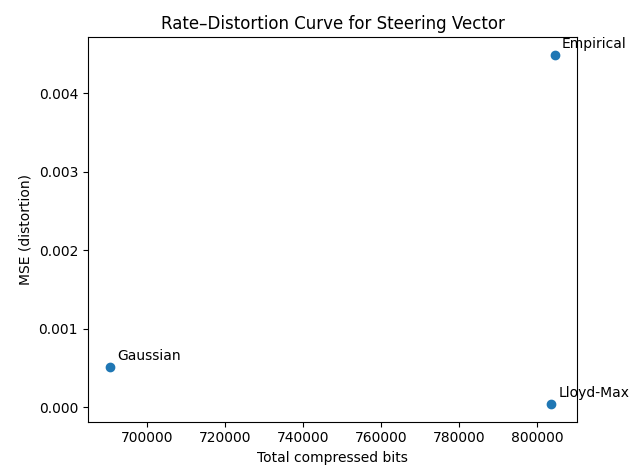
\includegraphics[width=0.5\textwidth]{Diagramm.png}
  \caption{Rate-distortion диаграмма}
  \label{fig:diagramm}
\end{figure}

Таким образом, при текущем объеме данных лучше всего сжимает steering vector гауссов приор. Но при увеличении объема данный есть вероятность, что выигрыш от точности восстановления steering vector с помощью Lloyd–Max превысит затраты на передачу метаданных.

\section*{Выводы}

\begin{itemize}
  \item Мы рассмотрели арифметическое кодирование текста на базе LLM. Нами были рассмотрены модели размером 70m-7b. Чем больше модель, тем лучший коэффициент сжатия она обеспечивает. Но большие модели работают медленнее и требуют больших вычислительных ресурсов.
  \item Предобученный steering vector способен улучшить коэффициент сжатия на несколько процентов. Необученный steering vector использовать нет смысла.
  \item Получившийся steering vector в целях дальнейшей оптимизации можно сам сжать, использую подход на основе hyper prior. Для лучшего коэффициента сжатия steering vector при малом объеме данных лучше использовать гауссов гипер-приор, а для лучшей точности восстановления steering vector - Lloyd–Max гипер‑приор.
\end{itemize}

\end{document}
